%%%%%%%%%%%%%%%%%%%%%%%%%%%%%%%%%%%%%%%%%%%%
% Modèle du projet %%%%%%%%%%%%%%%%%%%%%%%%%
% Cours d’Introduction à la Physique Quantique
% Université Nationale Autonome du Mexique %%
% Réalisé par Sergio Alfonso Pelayo Escalera %
%%%%%%%%%%%%%%%%%%%%%%%%%%%%%%%%%%%%%%%%%%%%
\documentclass[10pt]{article}
%%
\usepackage{adjustbox}
\usepackage{ulem}
\usepackage{tikz}
\usetikzlibrary{arrows.meta, positioning}
%%%
\usepackage{adjustbox}
\usepackage{array}
\usepackage{colortbl}
\usepackage{xcolor}
\usepackage{booktabs}
\usepackage{pifont} % pour les puces
\definecolor{rules}{RGB}{230,235,245}
\definecolor{stats}{RGB}{230,240,230}
\definecolor{erp}{RGB}{250,235,215}

\definecolor{rulesDot}{RGB}{60,90,150}
\definecolor{statsDot}{RGB}{60,120,80}
\definecolor{erpDot}{RGB}{200,130,40}
%%%
\usepackage{tikz}
\usetikzlibrary{arrows.meta, positioning}
\usepackage{graphicx}
\usepackage{float}
\usepackage{caption}
%\citestyle{numeric}
%%
\usepackage{tikz}
\usepackage{forest}
\usepackage{pgfplots}
\usepackage{amsmath}
\pgfplotsset{compat=1.18}
\usetikzlibrary{arrows.meta, positioning, shapes.geometric}
%%
\usepackage[utf8]{inputenc}
\usepackage{fontspec}
\setmainfont{Times New Roman}
%\usepackage[T1]{fontenc}
\usepackage{tcolorbox}
%\usepackage[russian,english]{babel}
\usepackage[french,english]{babel}
\usepackage[utf8]{inputenc}
\usepackage[french]{babel}
\usepackage{url}
\usepackage{hyperref}
\usepackage{amsmath}
\usepackage{amsfonts}
\usepackage{amssymb}
\usepackage{graphicx}
\usepackage{float}
\usepackage{lipsum}
\usepackage{multicol}
\usepackage{xcolor}
\usepackage{braket}
\usepackage{cancel}
\newcommand{\celda}[1]{
	\begin{minipage}{2.5cm}
		\vspace{5mm}
		#1
		\vspace{5mm}
	\end{minipage}
}
\definecolor{verde}{rgb}{0.24, 0.58, 0.26}
\usepackage[left=2.00cm, right=2.00cm, top=2.00cm, bottom=2.00cm]{geometry}
\author{El Argoubi El Mehdi}
\title{Détection d’Anomalies Explicables dans les Systèmes d’Information : État de l’Art et Application aux Systèmes de Pointage et de Paie}


\usepackage{tcolorbox}
\renewenvironment{abstract}
{
  \begin{center}
  \begin{tcolorbox}[
    colback=gray!10,
    colframe=white,
    width=\textwidth,
    boxrule=0pt
  ]
  \begin{center}
  \Large\bfseries \abstractname
  \end{center}
  \par\medskip
}
{
  \end{tcolorbox}
  \end{center}
}
\makeatother
%Header Footer

\usepackage{fancyhdr}

% Désactiver le style ACM
\pagestyle{fancy}
\fancyhf{}  % clear all header and footer fields

% Header
\fancyhead[L]{\textit{École d'Ingénieurs du Littoral-Côte-d'Opale}}
\fancyhead[R]{\textit{EDUREKA}}

% Footer
\fancyfoot[L]{\textit{El Argoubi El Mehdi}}
\fancyfoot[R]{\thepage}

% Supprimer la ligne horizontale du header (optionnel)
\renewcommand{\headrulewidth}{0.4pt}
\renewcommand{\footrulewidth}{0.4pt}

%couleur lien numero
\hypersetup{
    colorlinks=true,
    linkcolor=blue,
    citecolor=blue,
    urlcolor=blue
}
%
\usepackage{graphicx}
\usepackage{xcolor}
\usepackage{geometry}
\usepackage{multicol}
\usepackage{tcolorbox}
\usepackage{titlesec}
\usepackage{setspace}

\geometry{margin=2cm}

\definecolor{journalblue}{RGB}{0,70,140}
\definecolor{headergray}{RGB}{220,225,230}
%%


\fancypagestyle{firstpage}{
    \fancyhf{} % vide header et footer
    \fancyfoot[L]{\textit{El Argoubi El Mehdi}}
    \fancyfoot[R]{\thepage}
    \renewcommand{\headrulewidth}{0pt}   % supprime ligne du header
    \renewcommand{\footrulewidth}{0.4pt} % garde ligne du footer
}


\begin{document}
\thispagestyle{firstpage}
%%%%%%%%hnaaaaaaaaaaaa
%%

%------------------------------------------------
% HEADER JOURNAL STYLE
%------------------------------------------------
%------------------------------------------------
% TOP BLUE BAR
%------------------------------------------------

\vspace*{-1.2cm}
\noindent
\colorbox{journalblue}{%
\makebox[\dimexpr\textwidth-2\fboxsep\relax][c]{%
\parbox[c][0.25cm][c]{\textwidth}{%
\centering
\color{white}\bfseries\small
E. EL ARGOUBI / UNIVERSITY OF LITTORAL COTE D’OPALE / 2026
}}}

\vspace{0.1cm}

\noindent
\begin{minipage}{0.25\textwidth}

\includegraphics[width=1\linewidth]{eilco.png}
\end{minipage}
\hfill
\colorbox{white}{
\begin{minipage}{0.4\textwidth}
\centering
\vspace{2pt}

%{\bfseries\large ÉTUDE BIBLIOGRAPHIQUE}\\[6pt]

%{\color{blue}\small Cycle Ingénieur en Informatique 
%\\Parcours Data Science\small 
%}\\[6pt]
%{\small 2025--2026}
\vspace{2pt}
\end{minipage}
}
\hfill
\begin{minipage}{0.35\textwidth}

\includegraphics[width=1\linewidth]{Logo-ulco.png}
\end{minipage}

\vspace{0.1cm}

{\noindent\color{journalblue}\rule{\textwidth}{0.1cm}}


%\begin{center}
%\textbf{\uline{ÉTUDE BIBLIOGRAPHIQUE}}
%\end{center}
%------------------------------------------------

%------------------------------------------------
% TITLE
%------------------------------------------------
\vspace{0.4cm}

{\itshape\color{gray} \noindent \uline{Research Article}}

\vspace{0.3cm}

%\begin{center}
{
\LARGE \noindent
\textbf{DÉTECTION D’ANOMALIES EXPLICABLES DANS LES SYSTÈMES D’INFORMATION
ÉTAT DE L’ART ET APPLICATION AUX SYSTÈMES DE POINTAGE ET DE PAIE}\par
}
%\end{center}


\vspace{0.5cm}

%------------------------------------------------
% AUTHORS
%------------------------------------------------

%\begin{tabular}{l l l}
%    \textbf{ Auteur :}& EL ARGOUBI El Mehdi & \textbf{Email :} \textit{el-mehdi.el-argoubi@etu.eilco.univ-littoral.fr\\ }
% \end{tabular}

{\color{journalblue}\noindent \bfseries\scshape \Large
EL ARGOUBI El Mehdi
}
{\itshape \color{gray} \noindent \\
Engineering School of the Littoral Côte d’Opale, University of the Littoral Côte d’Opale, Calais 62100, France
}

\vspace{0.4cm}
{\color{journalblue}\hrule}
\vspace{0.4cm}

%------------------------------------------------
% TITRES SUR LA MEME LIGNE AVEC LIGNES SEPAREES
%------------------------------------------------
%------------------------------------------------
% TITRES SUR LA MEME LIGNE (EN BLEU)
%------------------------------------------------

\begin{minipage}[t]{0.22\textwidth}
\centering
{\color{journalblue}\textbf{A R T I C L E \quad I N F O}}

\vspace{0.1cm}
{\color{journalblue}\rule{\linewidth}{0.6pt}}
\end{minipage}
\hfill
\begin{minipage}[t]{0.73\textwidth}
{\color{journalblue}\textbf{A B S T R A C T}}

\vspace{0.1cm}
{\color{journalblue}\rule{\linewidth}{0.6pt}}
\end{minipage}

\vspace{0.5cm}

%------------------------------------------------
% CONTENU (EN NOIR)
%------------------------------------------------

\color{black}

\begin{minipage}[t]{0.24\textwidth}
{\color{journalblue}
\textbf{Mots-clés:}

\vspace{0.3cm}

Information Systems\\
Fraud Detection\\
Explainable AI\\
Anomaly Detection\\
ERP\\
Human Resource Systems

\vspace{0.8cm}

%\textbf{Nombre de mots :} 2271
}
\end{minipage}
\hfill
\begin{minipage}[t]{0.74\textwidth}
{\color{journalblue}
Les systèmes d’information dédiés au pointage et à la paie jouent un rôle essentiel dans les organisations, car ils traitent des données sensibles ayant un impact direct sur les employés, la conformité réglementaire et la gouvernance financière. La fiabilité de ces données constitue ainsi un enjeu majeur pour les processus de gestion.

Ces systèmes sont néanmoins exposés à des anomalies résultant d’erreurs de saisie, d’incohérences ou de comportements frauduleux, susceptibles d’affecter la qualité des données et la confiance des utilisateurs. Les mécanismes de contrôle traditionnels montrent leurs limites face à la complexité croissante des données.

Dans ce contexte, la littérature s’oriente vers des approches automatiques de détection d’anomalies explicables. Toutefois, dans des domaines sensibles comme la paie, la détection seule est insuffisante et doit être complétée par des mécanismes d’explicabilité.

Cette étude propose un état de l’art des approches de détection d’anomalies explicables appliquées aux systèmes de pointage et de paie.
}
\end{minipage}

\vspace{0.5cm}
{\color{journalblue}\hrule}
%--
%\noindent\color{journalblue}\rule{\textwidth}{1pt}

%%

%%%%%%%%hnaaaaa
%%%%%%%%%%%%%%%%%%%%%%%%%%%%%%%%%%%%%%%%%%%%%%%%%%%%%%%%%%%%%%%%
%\newpage
%	\begin{center}
%		\textcolor{blue}{\rule{175mm}{0.2mm}}
%	\end{center}		
    \selectlanguage{english}
%	\begin{abstract}
%		Information systems dedicated to time tracking and payroll management play a critical role in modern organizations, as they process highly sensitive data with direct implications for employees, regulatory compliance, and financial governance. Due to their central position within human resource and financial systems, anomalies resulting from data entry errors, rule inconsistencies, or fraudulent behaviors may lead to significant operational and financial consequences.\\
%        Traditional control mechanisms, mainly based on fixed rules and manual audits, show clear limitations when faced with the growing volume and complexity of organizational data, reducing their ability to detect subtle or evolving anomalies. Consequently, the scientific literature increasingly focuses on automated anomaly detection approaches. However, in sensitive domains such as payroll management, detection alone is insufficient: explanations that are understandable, traceable, and auditable are required to ensure user trust and regulatory compliance.\\
%        This bibliographic study presents a structured state of the art of explainable anomaly detection approaches in information systems, with a particular focus on their applicability to time tracking and payroll systems.

%		\vspace{2mm}
%		\underline{\textbf{Keywords:}} \hspace{1mm} \textit{Anomaly Detection, Explainable Artificial Intelligence, Information Systems, Payroll \& Time Tracking Systems, ERP \& Human Resource Systems, Financial Fraud.}
%	\end{abstract}


%    \selectlanguage{french}
%	\begin{abstract}
%		Les systèmes d’information dédiés au pointage et à la paie jouent un rôle essentiel dans les organisations, car ils traitent des données sensibles ayant un impact direct sur les employés, la conformité réglementaire et la gouvernance financière. La fiabilité de ces données constitue ainsi un enjeu majeur pour les processus de gestion.\\
%        Ces systèmes sont néanmoins exposés à des anomalies résultant d’erreurs de saisie, d’incohérences ou de comportements frauduleux, susceptibles d’affecter la qualité des données et la confiance des utilisateurs. Les mécanismes de contrôle traditionnels, fondés sur des règles fixes et des vérifications manuelles, montrent leurs limites face à la complexité croissante des données.\\
%        Dans ce contexte, la littérature s’oriente vers des approches automatiques de détection d’anomalies. Toutefois, dans des domaines sensibles comme la paie, la détection seule est insuffisante et doit être complétée par des mécanismes d’explicabilité afin de fournir des alertes compréhensibles, traçables et auditables, essentielles à la prise de décision et à la confiance des utilisateurs.\\
%        Cette étude propose un état de l’art des approches de détection d’anomalies explicables appliquées aux systèmes de pointage et de paie.

	%	\vspace{2mm}
	%	\textbf{Mots-clés:} \hspace{1mm} \textit{Détection d’anomalies, Intelligence artificielle explicable, Systèmes d’information, Systèmes de paie et de pointage, ERP \& systèmes RH, Fraude financière.}

	%\end{abstract}


    

%	\begin{center}
%		\textcolor{blue}{\rule{175mm}{0.2mm}}
%	\end{center}		

	\vspace{3mm}
	
	\begin{multicols}{2}
		\section*{Introduction}
            Les systèmes d’information sont essentiels aux processus de gestion des organisations, en particulier les systèmes de pointage et de paie, qui traitent des données sensibles liées au temps de travail et à la rémunération des employés, nécessitant une forte fiabilité pour assurer la conformité réglementaire et la gouvernance financière \cite{ref1,ref2,ref3}. Ces systèmes peuvent toutefois être affectés par des anomalies issues d’erreurs, d’incohérences ou de comportements anormaux, entraînant des dysfonctionnements tels que des retards de paiement. Dans ce contexte, les mécanismes de contrôle traditionnels, fondés sur des règles fixes et des vérifications manuelles, atteignent leurs limites face à la complexité croissante des données et des systèmes d’information \cite{ref2}, \cite{ref3}.\\
            Dans ce contexte, la détection automatique d’anomalies apparaît comme une approche prometteuse pour renforcer les mécanismes de contrôle des données de gestion. Néanmoins, dans des domaines sensibles comme la paie, la simple identification d’une anomalie ne suffit pas. Les utilisateurs doivent pouvoir comprendre les raisons à l’origine des alertes afin de prendre des décisions éclairées et justifiables. L’explicabilité des anomalies constitue ainsi un enjeu central pour renforcer la confiance des utilisateurs et assurer l’auditabilité des systèmes de détection automatique \cite{ref4}, \cite{ref5}.\\
            L’objectif de cette recherche bibliographique est de proposer un état de l’art structuré des approches de détection d’anomalies explicables dans les systèmes d’information, et d’analyser leur pertinence pour les systèmes de pointage et de paie.

            \begin{center}
            \centering
                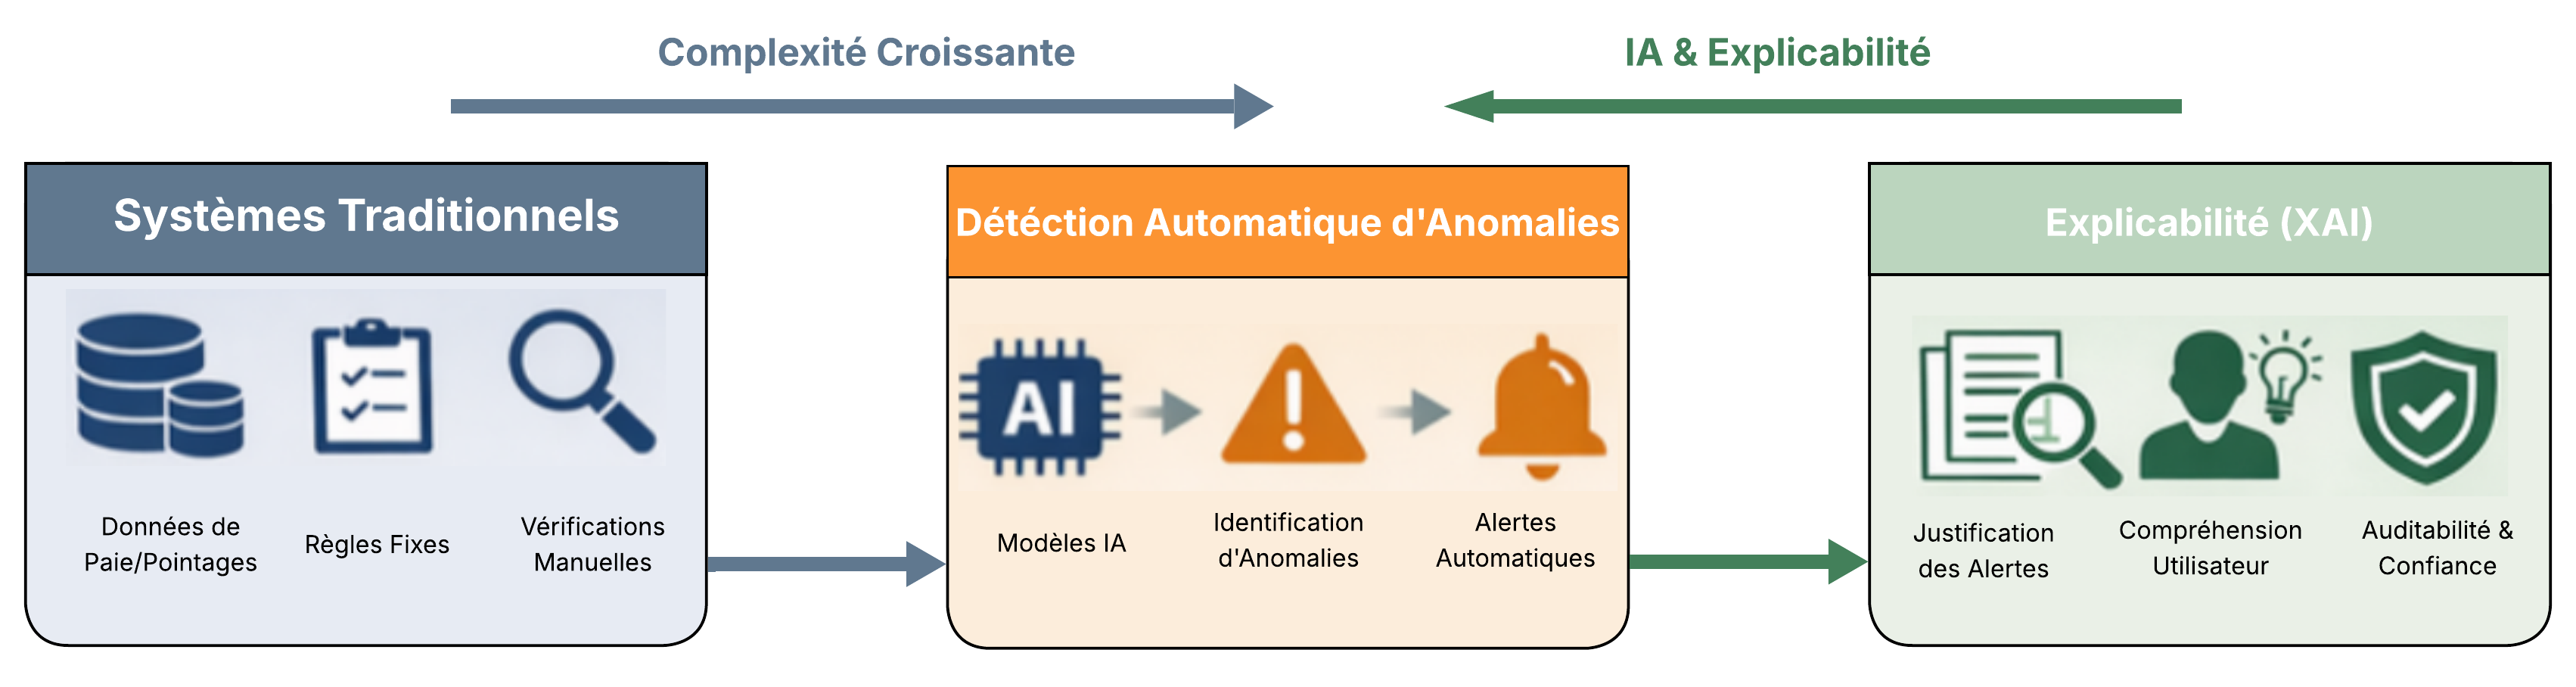
\includegraphics[width=1\linewidth]{Transition.png}
                \captionof{figure}{Transition des contrôles traditionnels vers la détection d’anomalies explicable}
            \end{center}
%%%%%%%%

		\section{Détection d’anomalies : concepts et enjeux}
            \subsection{Définition des anomalies}
            Dans les systèmes de gestion, une anomalie correspond à un écart par rapport au fonctionnement attendu, tel que défini par les données historiques, les règles métier ou les processus organisationnels, cette normalité étant dépendante du contexte applicatif \cite{ref6}, \cite{ref7}.\\
            Il est essentiel de distinguer l’anomalie d’autres notions proches : l’erreur, généralement non intentionnelle et liée à la saisie ou au traitement des données \cite{ref8} ; l’incohérence, résultant d’une contradiction entre informations ou règles métier \cite{ref9} ; et la fraude, qui implique une violation intentionnelle des règles à des fins de gain \cite{ref2}, \cite{ref10}.\\
            L’anomalie constitue ainsi un signal d’alerte générique, sans présumer de la cause ou de l’intention, visant à attirer l’attention des acteurs humains sur des situations nécessitant une analyse approfondie, ce qui justifie l’importance de mécanismes de détection fiables et interprétables \cite{ref11}.
            \subsection{Typologies d’anomalies}
            La littérature distingue trois grandes catégories d’anomalies dans les systèmes de gestion. Les anomalies statistiques correspondent à des valeurs numériques atypiques par rapport à un comportement de référence, fréquemment observées dans les données transactionnelles et temporelles \cite{ref8}, \cite{ref10}. Les anomalies comportementales concernent des schémas d’actions ou des profils d’utilisation inhabituels, détectables par analyse temporelle ou par comparaison entre entités similaires \cite{ref12}, \cite{ref2}. Enfin, les anomalies logiques résultent de violations de règles ou de contraintes métier, même lorsque les valeurs prises individuellement paraissent cohérentes \cite{ref7}, \cite{ref9}.\\
            Cette typologie montre que la détection d’anomalies repose à la fois sur l’analyse des données, des comportements et des règles métier, en particulier dans les systèmes ERP ainsi que dans les systèmes de pointage et de paie \cite{ref7}, \cite{ref6}.

            \begin{center}
            \centering
                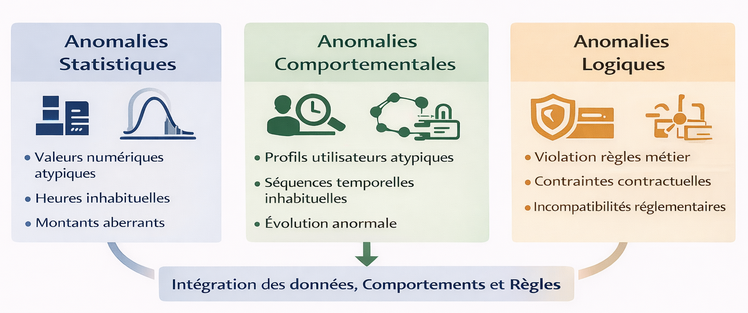
\includegraphics[width=1\linewidth]{TypologieAnomalies.png}
                \captionof{figure}{Typologie des anomalies dans les systèmes ERP}
            \end{center}

            

        \section{Approches de détection d’anomalies dans les systèmes de gestion}
        La littérature scientifique distingue plusieurs familles d’approches pour la détection d’anomalies dans les systèmes de gestion, différant par leur niveau d’automatisation, leur adaptabilité et leur capacité d’interprétation. Ces approches sont généralement regroupées en trois catégories : approches basées sur des règles, approches statistiques et exploratoires, et approches avancées appliquées aux systèmes ERP, le choix dépendant fortement des exigences d’explicabilité et d’auditabilité du contexte applicatif \cite{ref13}.

        \begin{center}
            \centering
            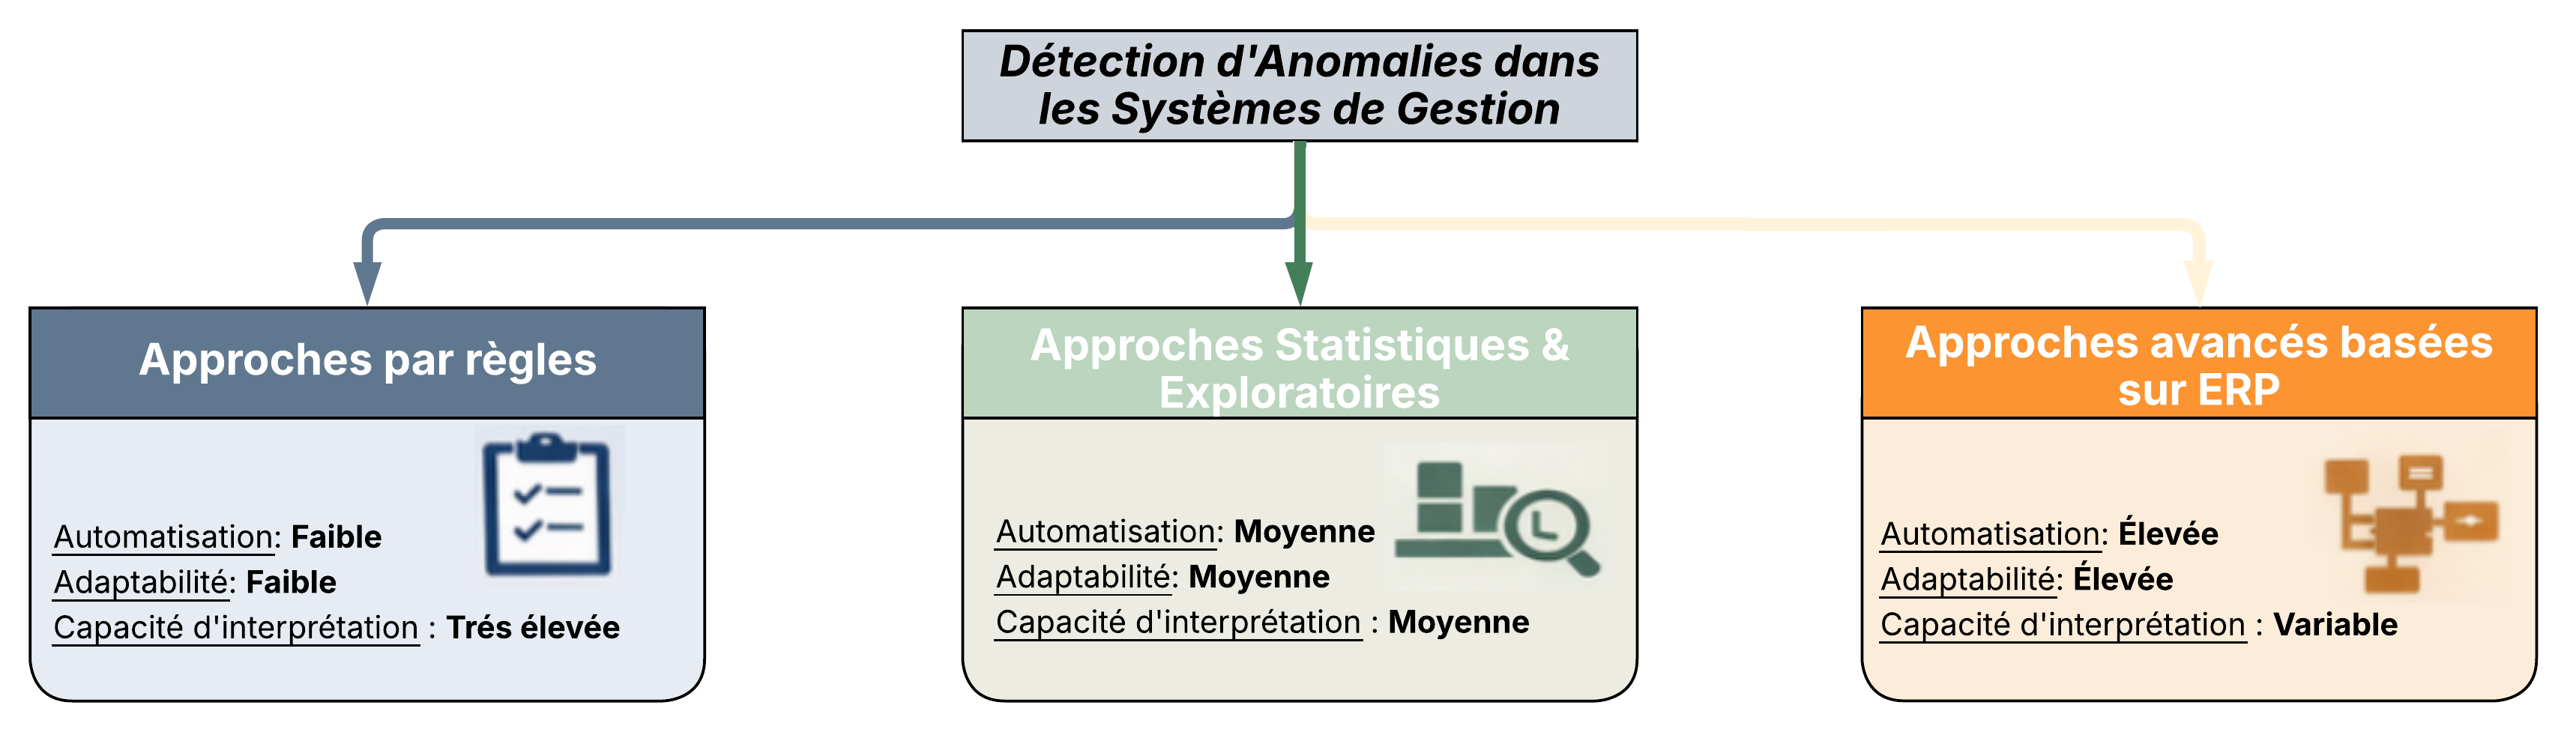
\includegraphics[width=1\linewidth]{Approches_détection.png}
            \captionof{figure}{Approches de détection d’anomalies dans les systèmes d’information}
        \end{center}
            \subsection{Approches basées sur des règles}
            Les approches basées sur des règles constituent le premier niveau historique de contrôle dans les systèmes d’information de gestion. Elles reposent sur la formalisation explicite de règles métier issues de cadres réglementaires ou organisationnels, définissant les conditions normales de fonctionnement des processus administratifs et financiers \cite{ref1}.\\
            Dans les systèmes de pointage et de paie, ces règles permettent de vérifier la cohérence des heures déclarées et la conformité des calculs de rémunération \cite{ref2}, \cite{ref3}. Leur principal avantage réside dans leur simplicité, leur transparence et leur facilité d’audit, les règles étant directement compréhensibles par les utilisateurs métier \cite{ref4}.\\
            Cependant, ces approches sont peu adaptées à l’évolution des comportements, difficiles à maintenir à grande échelle et inefficaces pour détecter des anomalies nouvelles ou subtiles. Elles peuvent également générer un nombre élevé de faux positifs dans des environnements complexes et dynamiques \cite{ref10}, \cite{ref13}, ce qui a motivé le développement d’approches plus flexibles et orientées données.

            \subsection{Approches statistiques et exploratoires}
            Les approches statistiques détectent les anomalies en identifiant des valeurs atypiques par rapport à un comportement de référence, à partir de l’analyse des distributions de données. Elles sont particulièrement adaptées aux données tabulaires et numériques présentes dans les systèmes de gestion, notamment les données de pointage et de paie \cite{ref6}.\\
            Ces méthodes permettent de repérer des écarts significatifs sur des variables telles que les heures travaillées ou les montants de rémunération \cite{ref8}. L’analyse de profils prolonge cette approche en comparant le comportement d’une entité à celui d’un groupe de référence afin d’identifier des anomalies persistantes \cite{ref12}.\\
            Cependant, ces approches fournissent le plus souvent des explications limitées, indiquant principalement qu’une valeur est atypique. Certains travaux proposent d’y associer des mécanismes d’explication post-hoc afin de préciser le rôle des variables dans l’anomalie détectée \cite{ref14}. Malgré cela, leur dépendance aux seuils et à une normalité définie par le contexte limite leur robustesse et leur interprétabilité dans des domaines sensibles comme la paie \cite{ref10}.

            \subsection{Approches avancées appliquées aux ERP}
            Dans les systèmes ERP, la détection d’anomalies s’appuie de plus en plus sur l’analyse des journaux transactionnels et des traces d’exécution des processus métier \cite{ref7}. Ces approches modélisent les séquences d’événements, les dépendances entre modules et les comportements utilisateurs afin de détecter des anomalies de processus plutôt que de simples valeurs aberrantes.\\
            L’analyse des journaux ERP permet d’identifier des séquences de transactions atypiques, des violations de flux de processus ou des comportements utilisateurs incohérents dans le temps \cite{ref2}, \cite{ref12}. Toutefois, la complexité et l’hétérogénéité des données ERP rendent l’interprétation des anomalies difficile, nécessitant des mécanismes d’explicabilité capables de relier les anomalies détectées aux étapes du processus ou aux règles métier concernées \cite{ref15}.\\
        \begin{center}
            \centering
            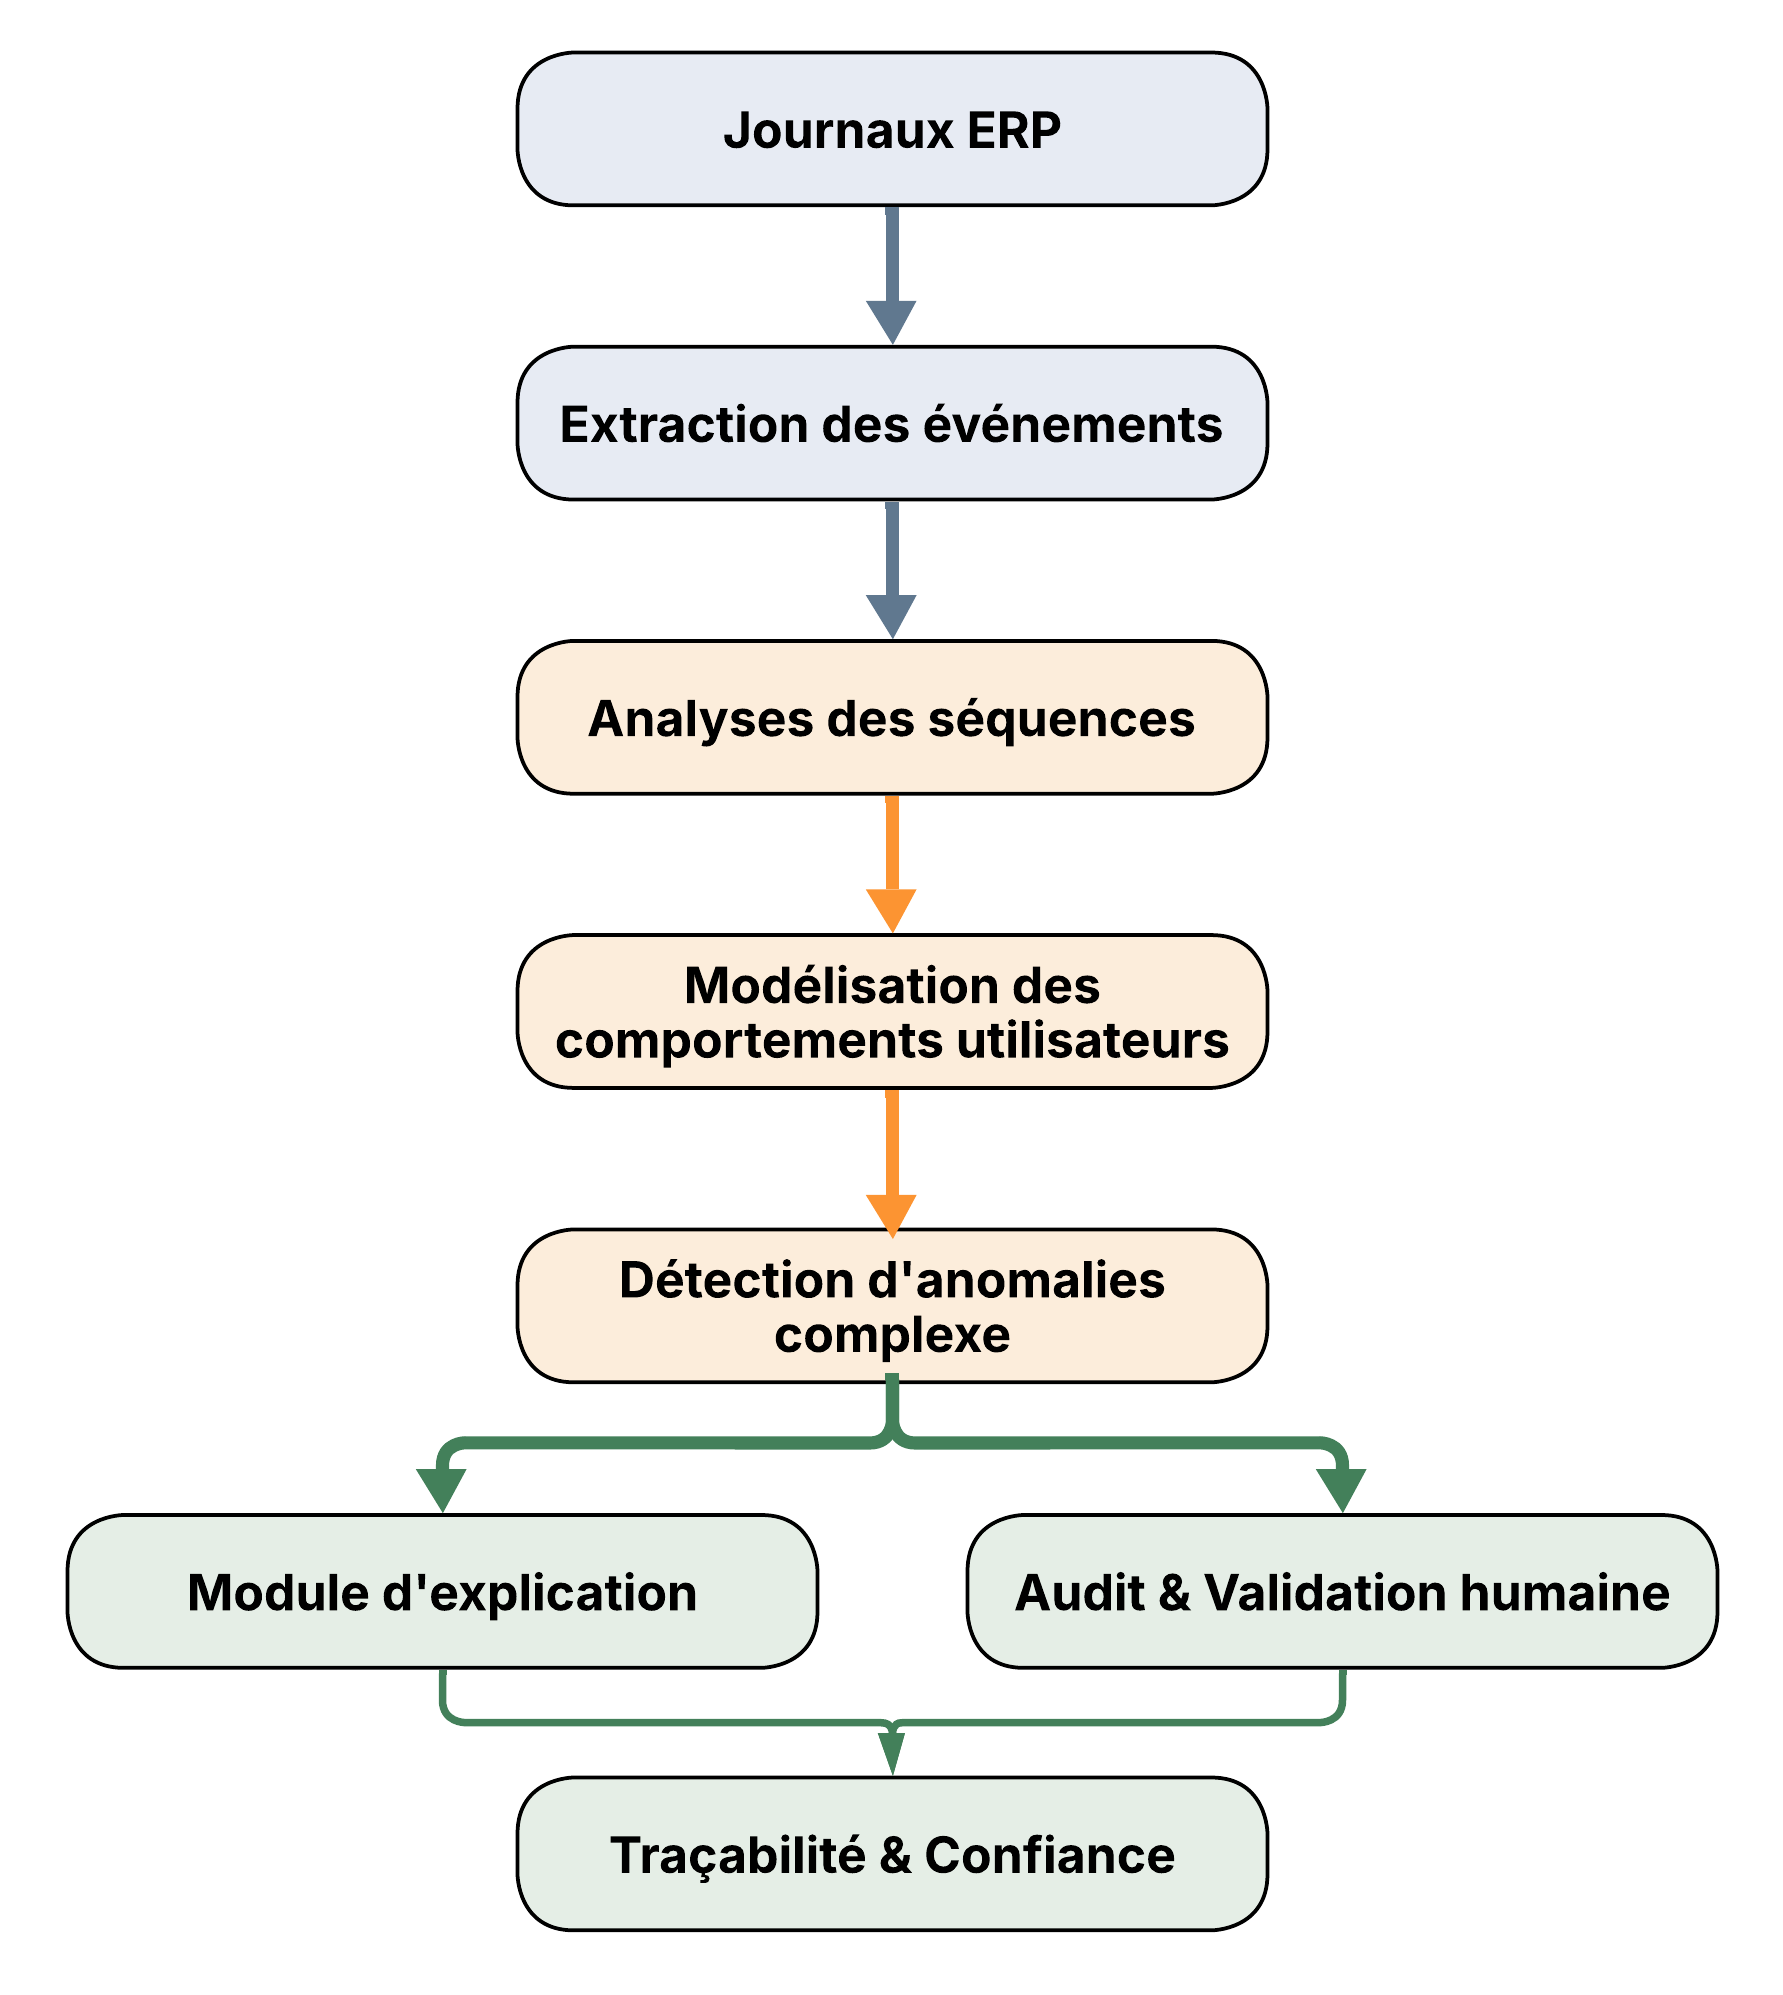
\includegraphics[width=0.9\linewidth]{journal.png}
            \captionof{figure}{Détection d’anomalies basée sur l’analyse des journaux ERP}
        \end{center}

            Ces approches offrent une meilleure capacité de détection mais renforcent la nécessité d’outils explicables, en particulier dans les contextes de paie où chaque anomalie doit être justifiée de manière précise et traçable \cite{ref11}, \cite{ref7}, \cite{ref3}.

%%
\begin{center}

\renewcommand{\arraystretch}{1.3}
\setlength{\tabcolsep}{5pt} % réduit l’espace entre colonnes

\begin{adjustbox}{max width=\linewidth}
\begin{tabular}{>{\bfseries}l
                >{\columncolor{rules}}c
                >{\columncolor{stats}}c
                >{\columncolor{erp}}c}

\toprule
 & Approches par règles 
 & Statistiques 
 & Avancées ERP \\

\midrule
Automatisation & Faible & Moyenne & Élevée \\
Adaptabilité & Faible & Moyenne & Élevée \\
Détection anomalies nouvelles & Faible & Moyenne & Élevée \\
Interprétabilité & Très élevée & Moyenne & Variable \\
Complexité & Faible & Moyenne & Élevée \\
Auditabilité & Forte & Moyenne & Forte si explicable \\

\bottomrule
\end{tabular}
\end{adjustbox}

\captionof{table}{Comparaison des approches de détection d’anomalies}
\end{center}
%%
            
        \section{Explicabilité des anomalies}
            \subsection{Pourquoi expliquer une anomalie ?}
            Dans les systèmes de gestion critiques, une alerte non expliquée est difficilement exploitable. L’explicabilité permet de transformer une détection automatique en information actionnable, en identifiant les facteurs ayant conduit à l’anomalie et en facilitant l’analyse humaine \cite{ref4}, \cite{ref5}.\\
            L’explicabilité contribue également à assurer la traçabilité et l’auditabilité des décisions automatiques, ce qui est essentiel dans des domaines sensibles comme la paie et le pointage \cite{ref4}. Enfin, l’explicabilité favorise l’acceptation des systèmes de détection et facilite l’intégration d’une validation humaine dans le processus décisionnel \cite{ref16}.

        \begin{center}

\begin{adjustbox}{max width=\linewidth}
\begin{tikzpicture}[
    node distance=0.2cm and 0.3cm,
    boxGreen/.style={
        rectangle,
        rounded corners,
        minimum width=4.2cm,
        minimum height=3.2cm,
        text width=3.8cm,
        fill=green!20,
        draw=none,
        align=center
    },
    boxBlue/.style={
        rectangle,
        rounded corners,
        minimum width=4.2cm,
        minimum height=3.2cm,
        text width=3.8cm,
        fill=blue!20,
        draw=none,
        align=center
    }
]

% Ligne 1
\node[boxGreen] (c) {
\textbf{Compréhension}\\[8pt]
Permet d’expliquer les alertes à l’utilisateur pour faciliter la compréhension.
};

\node[boxGreen, right=of c] (a) {
\textbf{Amélioration}\\[8pt]
Aide à affiner les modèles et les règles de détection au fil du temps.
};

% Ligne 2
\node[boxBlue, below=of c] (au) {
\textbf{Auditabilité}\\[8pt]
Facilite le suivi des alertes et des décisions à des fins de vérification.
};

\node[boxBlue, right=of au] (p) {
\textbf{Protection juridique}\\[8pt]
Offre une défense juridique en cas de litige ou de contrôle réglementaire.
};

\end{tikzpicture}
\end{adjustbox}

\captionof{figure}{Bénéfices de l’explicabilité}
\label{fig:explicabilite}

\end{center}

            \subsection{Types d’explications proposés dans la littérature}
            La littérature distingue plusieurs familles de méthodes d’explicabilité appliquées à la détection d’anomalies. Les approches post-hoc, telles que LIME et SHAP, sont largement utilisées pour expliquer des modèles complexes, et les modèles intrinsèquement explicables.\\
            LIME repose sur une approximation locale du modèle en construisant un modèle interprétable autour de l’observation anormale, permettant d’identifier les variables les plus influentes localement, tandis que SHAP s’appuie sur la théorie des valeurs de Shapley et attribue à chaque variable une contribution additive à la décision, offrant une mesure quantitative et cohérente de l’influence des attributs sur la détection \cite{ref4}, \cite{ref6}, \cite{ref11}.\\
            En parallèle, les modèles intrinsèquement explicables, tels que les modèles à base de règles, de contraintes logiques ou les approches hybrides combinant logique symbolique et apprentissage, permettent d’intégrer l’explicabilité directement dans le processus de détection. Ces modèles relient explicitement une anomalie à une violation de règles métier ou de contraintes, ce qui est particulièrement adapté aux systèmes ERP et de paie soumis à des exigences réglementaires fortes \cite{ref7}, \cite{ref9}.\\
            Enfin, la littérature distingue les explications globales, décrivant le comportement général du modèle, et les explications locales, centrées sur une alerte précise. Les explications locales sont privilégiées dans les systèmes de pointage et de paie, où chaque anomalie doit être analysée et validée individuellement \cite{ref5}, \cite{ref6}.

        \subsection{Apports et limites des approches explicables}
        Les approches explicables améliorent la compréhension des alertes, facilitent leur validation humaine et renforcent la traçabilité des décisions automatiques, ce qui favorise leur intégration dans les processus d’audit et de contrôle \cite{ref5}, \cite{ref11}, \cite{ref3}.\\
        Cependant, la qualité des explications dépend fortement des modèles utilisés et du contexte applicatif. Un compromis persiste entre performance de détection et interprétabilité, et l’évaluation objective des explications reste un défi ouvert \cite{ref5}, \cite{ref6}. Ces limites confirment que l’explicabilité demeure un axe de recherche central dans les systèmes de gestion.

        
		\section{Application aux systèmes de pointage et de paie}
        Les systèmes de pointage et de paie reposent sur des données tabulaires, temporelles et fortement structurées issues des systèmes RH et ERP, combinant informations individuelles, contractuelles et réglementaires \cite{ref1}, \cite{ref2}. Cette dépendance aux règles métier rend la définition de la normalité fortement contextuelle, tandis que toute anomalie peut avoir des conséquences financières, sociales ou juridiques.\\
        Dans ces systèmes, les anomalies peuvent être de nature statistique, comme un volume d’heures travaillées inhabituellement élevé, ou comportementale, par exemple un recours récurrent aux heures supplémentaires sur certaines périodes \cite{ref12}. Les anomalies logiques sont particulièrement critiques en paie et résultent de violations explicites des règles métier, telles qu’un conflit entre heures supplémentaires et contrat de travail, l’attribution d’une prime non prévue par la convention collective, ou une incohérence entre le temps de présence et les absences déclarées \cite{ref7}, \cite{ref9}.\\
        Les exigences de fiabilité et de conformité imposent que ces anomalies soient détectées avant la validation finale de la paie \cite{ref3}, \cite{ref7}. Dans ce contexte, les approches de détection ne sont réellement efficaces que si elles sont accompagnées de mécanismes d’explication permettant de justifier les alertes auprès des acteurs métiers et des instances de contrôle \cite{ref4}, \cite{ref5}.\\
        Les approches explicables facilitent l’analyse et la validation des alertes en reliant les anomalies à des règles métier, des variables spécifiques ou des écarts comportementaux, réduisant ainsi le temps d’investigation \cite{ref7}, \cite{ref8}. Les explications locales sont particulièrement adaptées à la paie, où chaque alerte doit être examinée individuellement \cite{ref6}, \cite{ref11}. La littérature met également en avant l’importance d’une validation humaine pour limiter les faux positifs et renforcer l’acceptabilité des systèmes automatisés \cite{ref8}, \cite{ref12}, \cite{ref16}.\\
        Cependant, les travaux spécifiquement dédiés aux systèmes RH restent limités. Les approches existantes sont majoritairement transposées d’autres contextes ERP, sans adaptation complète aux spécificités des données de paie, notamment leur caractère mixte, temporel et réglementé \cite{ref2}, \cite{ref14}, \cite{ref15}.

        \begin{center}
            \centering
            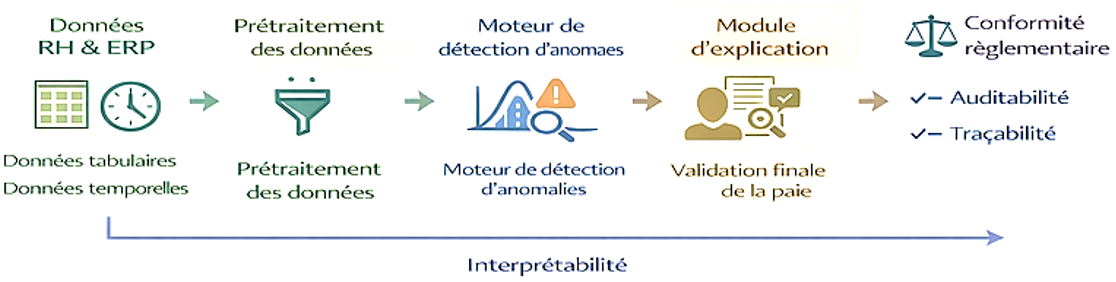
\includegraphics[width=1\linewidth]{flux.png}
            \captionof{figure}{Approche explicable de détection d’anomalies}
        \end{center}


		\section{Discussion et perspectives de recherche}
        La littérature montre que la détection automatique d’anomalies constitue un levier important pour le contrôle des systèmes d’information de gestion, en particulier dans les environnements ERP et RH caractérisés par des données complexes et interconnectées. Toutefois, dans des contextes sensibles comme le pointage et la paie, la détection seule est insuffisante et doit être complétée par des mécanismes permettant de comprendre et de justifier les alertes.\\
        L’explicabilité apparaît ainsi comme un élément central pour renforcer la confiance des utilisateurs, faciliter l’auditabilité et soutenir la prise de décision humaine. Néanmoins, des limites persistent, notamment les compromis entre performance de détection et interprétabilité, ainsi que la difficulté d’évaluer objectivement la qualité des explications.\\
        Les perspectives de recherche portent principalement sur l’amélioration de l’explicabilité pour des données mixtes et temporelles, l’intégration renforcée des règles métier et de la validation humaine, ainsi que le développement de cadres de détection pleinement auditables et conformes aux contraintes réglementaires des systèmes de gestion critiques.


        \section{Conclusion}
        Cette recherche bibliographique a présenté un état de l’art des approches de détection d’anomalies explicables dans les systèmes d’information, avec un focus sur les systèmes de pointage et de paie. La littérature montre que les approches traditionnelles et statistiques, bien qu’utiles, atteignent leurs limites face à la complexité croissante des données et des processus de gestion.\\
        Les approches avancées appliquées aux environnements ERP offrent de meilleures capacités de détection, mais renforcent la nécessité d’une explicabilité garantissant la compréhension, la confiance des utilisateurs et l’auditabilité des décisions, en particulier dans des contextes sensibles comme la paie. Enfin, les perspectives de recherche soulignent l’importance d’adapter les mécanismes d’explicabilité aux données mixtes et temporelles, d’intégrer davantage les règles métier et la validation humaine, et de développer des cadres de détection pleinement conformes aux contraintes réglementaires.





    \bigskip

    
    \bigskip
        \bibliographystyle{IEEEtran}
        \bibliography{references}
%%%%

	\end{multicols}

%    \bibliographystyle{IEEEtran}
%    \bibliography{references}









\end{document}